\documentclass{article}\usepackage[]{graphicx}\usepackage[]{color}
%% maxwidth is the original width if it is less than linewidth
%% otherwise use linewidth (to make sure the graphics do not exceed the margin)
\makeatletter
\def\maxwidth{ %
  \ifdim\Gin@nat@width>\linewidth
    \linewidth
  \else
    \Gin@nat@width
  \fi
}
\makeatother

\definecolor{fgcolor}{rgb}{0.345, 0.345, 0.345}
\newcommand{\hlnum}[1]{\textcolor[rgb]{0.686,0.059,0.569}{#1}}%
\newcommand{\hlstr}[1]{\textcolor[rgb]{0.192,0.494,0.8}{#1}}%
\newcommand{\hlcom}[1]{\textcolor[rgb]{0.678,0.584,0.686}{\textit{#1}}}%
\newcommand{\hlopt}[1]{\textcolor[rgb]{0,0,0}{#1}}%
\newcommand{\hlstd}[1]{\textcolor[rgb]{0.345,0.345,0.345}{#1}}%
\newcommand{\hlkwa}[1]{\textcolor[rgb]{0.161,0.373,0.58}{\textbf{#1}}}%
\newcommand{\hlkwb}[1]{\textcolor[rgb]{0.69,0.353,0.396}{#1}}%
\newcommand{\hlkwc}[1]{\textcolor[rgb]{0.333,0.667,0.333}{#1}}%
\newcommand{\hlkwd}[1]{\textcolor[rgb]{0.737,0.353,0.396}{\textbf{#1}}}%
\let\hlipl\hlkwb

\usepackage{framed}
\makeatletter
\newenvironment{kframe}{%
 \def\at@end@of@kframe{}%
 \ifinner\ifhmode%
  \def\at@end@of@kframe{\end{minipage}}%
  \begin{minipage}{\columnwidth}%
 \fi\fi%
 \def\FrameCommand##1{\hskip\@totalleftmargin \hskip-\fboxsep
 \colorbox{shadecolor}{##1}\hskip-\fboxsep
     % There is no \\@totalrightmargin, so:
     \hskip-\linewidth \hskip-\@totalleftmargin \hskip\columnwidth}%
 \MakeFramed {\advance\hsize-\width
   \@totalleftmargin\z@ \linewidth\hsize
   \@setminipage}}%
 {\par\unskip\endMakeFramed%
 \at@end@of@kframe}
\makeatother

\definecolor{shadecolor}{rgb}{.97, .97, .97}
\definecolor{messagecolor}{rgb}{0, 0, 0}
\definecolor{warningcolor}{rgb}{1, 0, 1}
\definecolor{errorcolor}{rgb}{1, 0, 0}
\newenvironment{knitrout}{}{} % an empty environment to be redefined in TeX

\usepackage{alltt}

\usepackage[british,russian]{babel} % выбор языка для документа
\usepackage[utf8]{inputenc} % задание utf8 кодировки исходного tex файла
\usepackage[X2,T2A]{fontenc}        % кодировка

\usepackage{fontspec}         % пакет для подгрузки шрифтов
\setmainfont{Arial}   % задаёт основной шрифт документа


\usepackage{float} % h h! H 

\usepackage{etoolbox}

\title{Отчёт о проделанной работе №1}
\author{Винни-Пух}
\date{\today}
\IfFileExists{upquote.sty}{\usepackage{upquote}}{}
\begin{document}

\maketitle




\section{Введение}

В этой замечательной работе мы выясним что было первым: курица или яйцо. 

\begin{knitrout}
\definecolor{shadecolor}{rgb}{0.969, 0.969, 0.969}\color{fgcolor}\begin{kframe}
\begin{alltt}
\hlkwd{library}\hlstd{(ggplot2)}
\hlkwd{head}\hlstd{(chickwts)}
\end{alltt}
\begin{verbatim}
##   weight      feed
## 1    179 horsebean
## 2    160 horsebean
## 3    136 horsebean
## 4    227 horsebean
## 5    217 horsebean
## 6    168 horsebean
\end{verbatim}
\end{kframe}
\end{knitrout}

\begin{knitrout}
\definecolor{shadecolor}{rgb}{0.969, 0.969, 0.969}\color{fgcolor}

{\centering 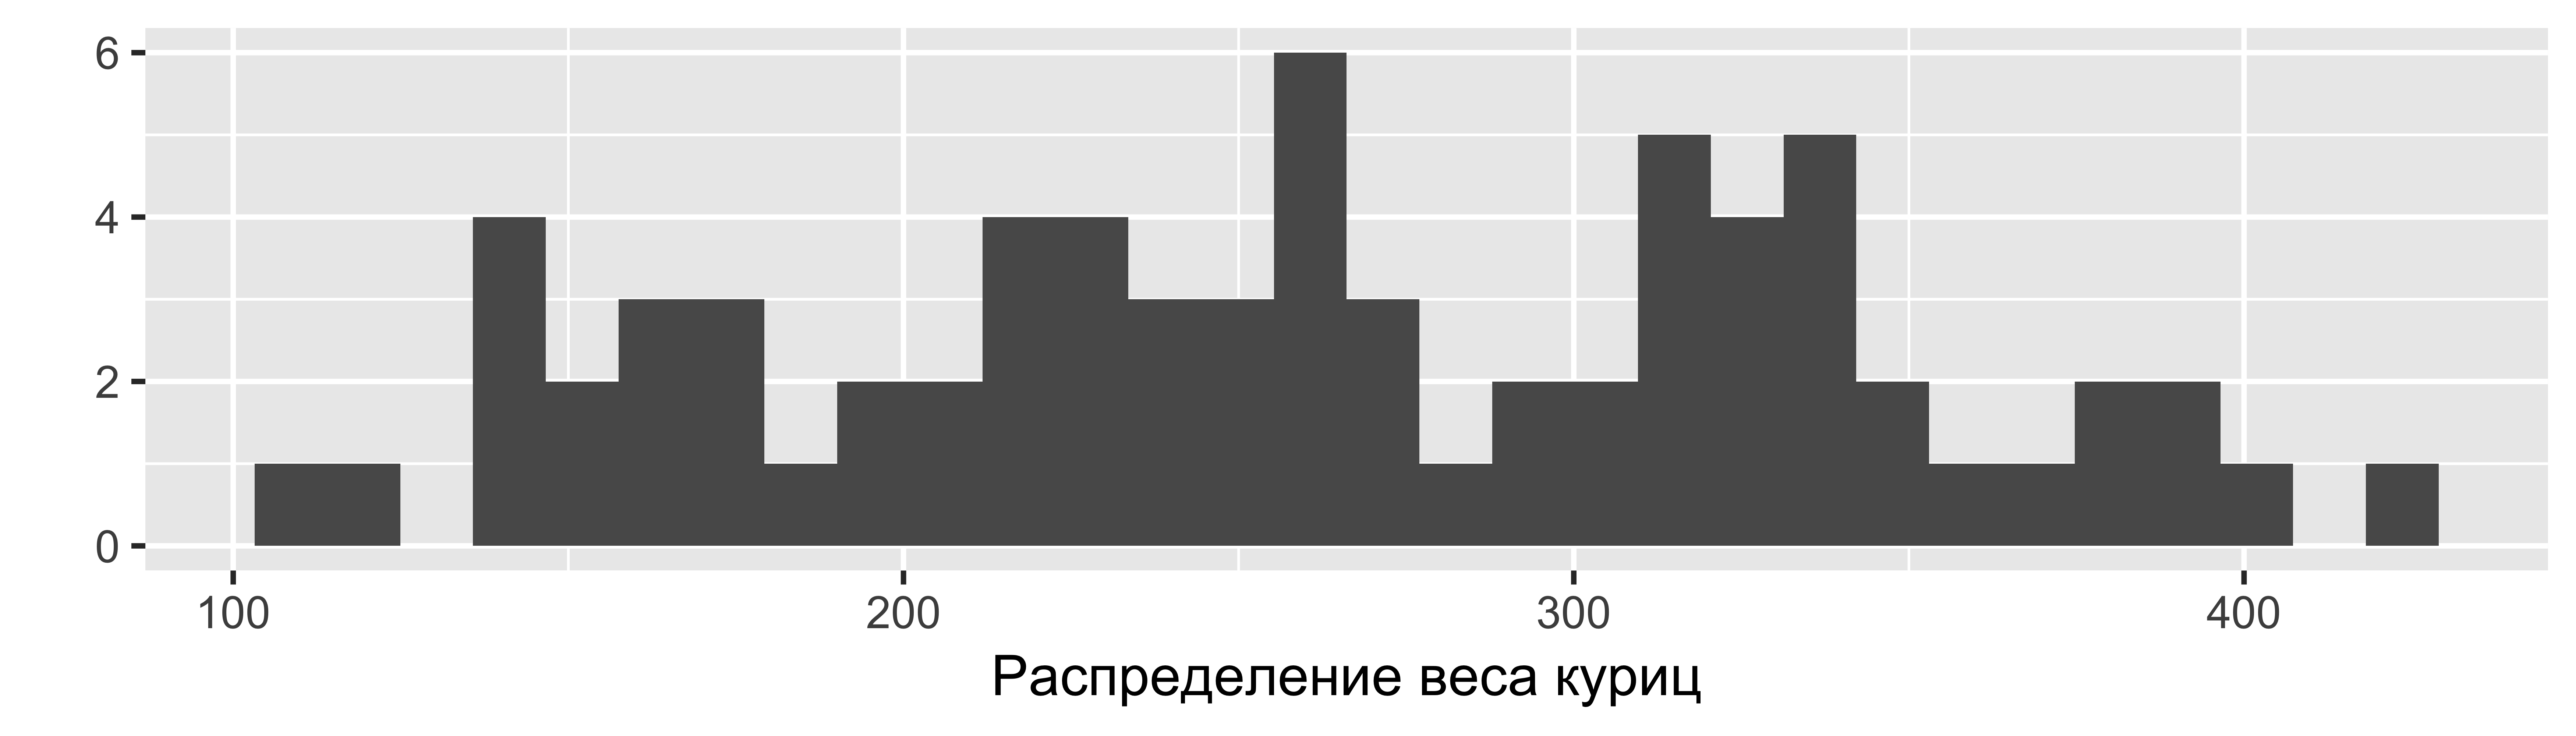
\includegraphics[width=\maxwidth]{figure/unnamed-chunk-3-1} 

}



\end{knitrout}

\section{Анализ данных}

Формула: 

\[ \int_{0}^{+\infty} x^{s-1} \cdot e^{-x} dx = \Gamma(s). \]



Среднее сегодня $0.12$


\section{Подпись картинки}

\begin{figure}[H]
\begin{knitrout}
\definecolor{shadecolor}{rgb}{0.969, 0.969, 0.969}\color{fgcolor}

{\centering 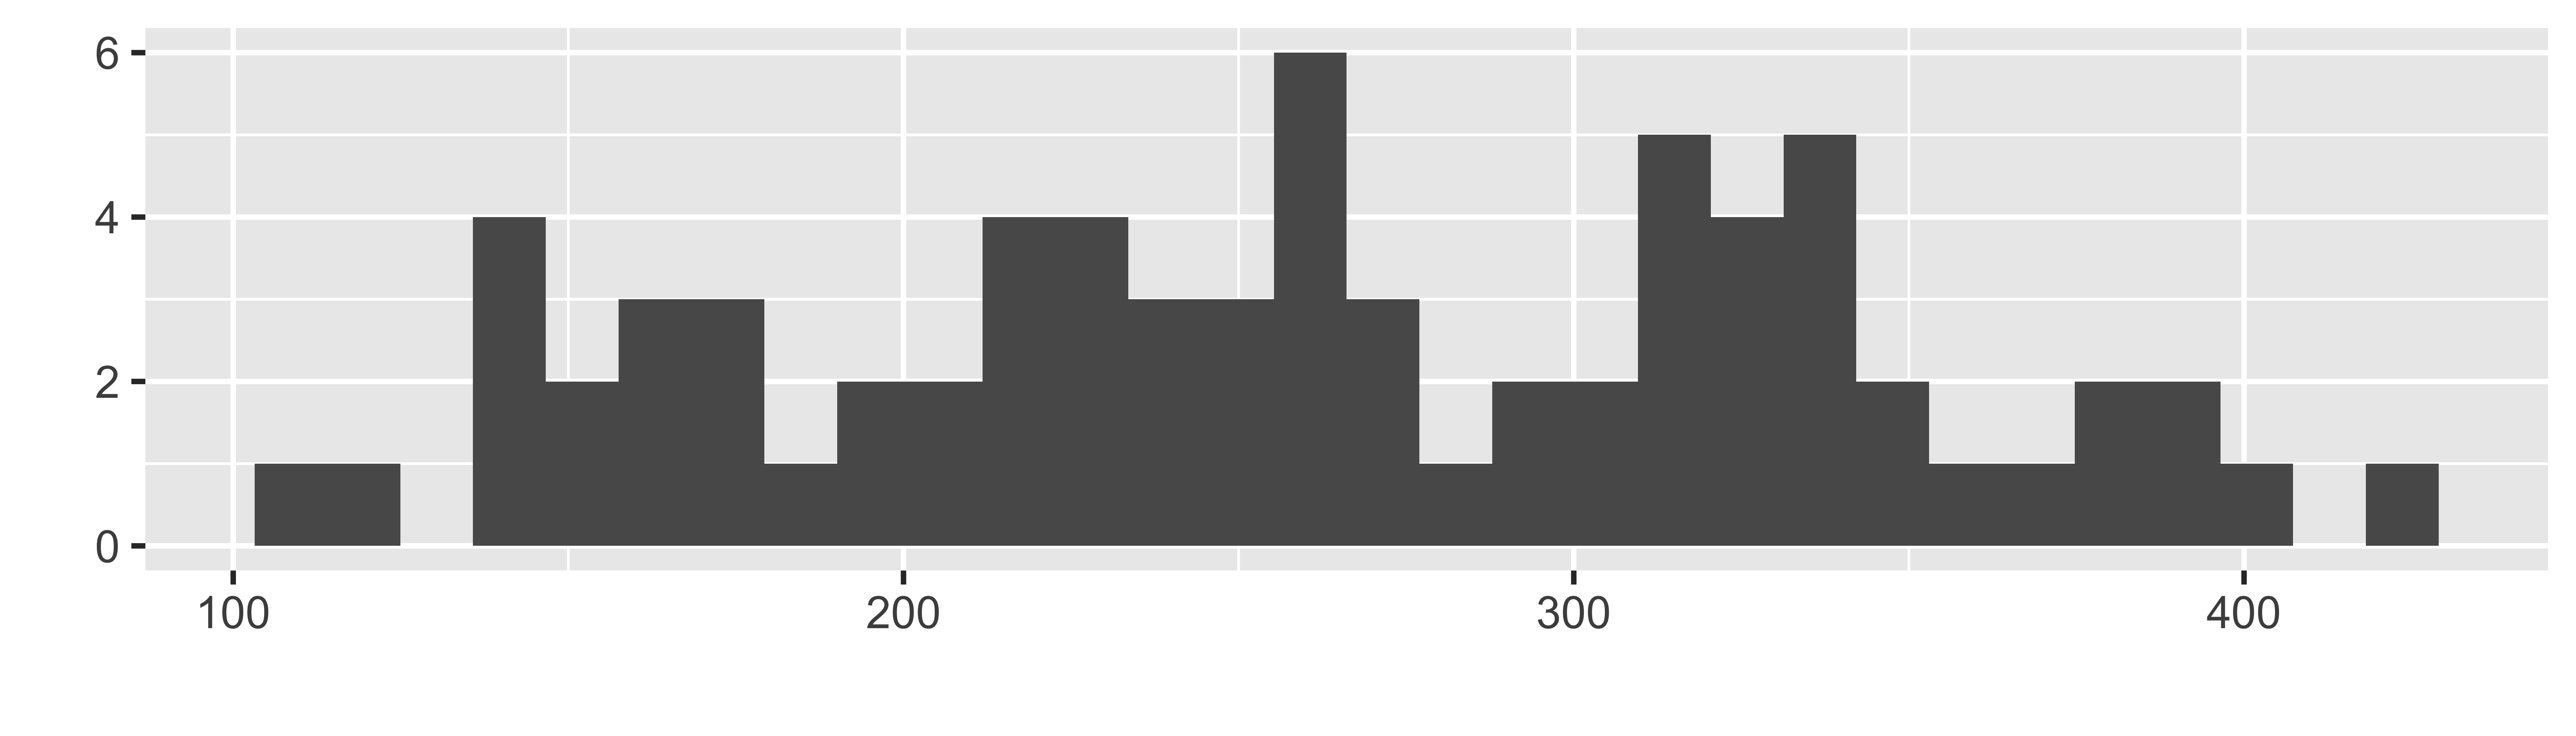
\includegraphics[width=\maxwidth]{figure/unnamed-chunk-5-1} 

}



\end{knitrout}
\caption{Вес куриц}
\end{figure}

\section{Модель}

Хотим оценить модель и посмотрерть на неё, а ещё есть хотим

\begin{knitrout}
\definecolor{shadecolor}{rgb}{0.969, 0.969, 0.969}\color{fgcolor}\begin{kframe}
\begin{verbatim}
## 
## Call:
## lm(formula = y ~ x)
## 
## Residuals:
##     Min      1Q  Median      3Q     Max 
## -149.40  -51.77   10.58   40.20  159.41 
## 
## Coefficients:
##             Estimate Std. Error t value Pr(>|t|)    
## (Intercept) 179.1268    15.0414  11.909  < 2e-16 ***
## x             2.2829     0.3631   6.287 2.54e-08 ***
## ---
## Signif. codes:  0 '***' 0.001 '**' 0.01 '*' 0.05 '.' 0.1 ' ' 1
## 
## Residual standard error: 62.7 on 69 degrees of freedom
## Multiple R-squared:  0.3642,	Adjusted R-squared:  0.355 
## F-statistic: 39.53 on 1 and 69 DF,  p-value: 2.537e-08
\end{verbatim}
\end{kframe}
\end{knitrout}


\begin{knitrout}
\definecolor{shadecolor}{rgb}{0.969, 0.969, 0.969}\color{fgcolor}\begin{kframe}
\begin{alltt}
\hlstd{y} \hlkwb{=} \hlstd{chickwts}\hlopt{$}\hlstd{weight}
\hlstd{x} \hlkwb{=} \hlnum{1}\hlopt{:}\hlkwd{length}\hlstd{(y)}
\hlkwd{qplot}\hlstd{(x, y,} \hlkwc{geom}\hlstd{=}\hlstr{'line'}\hlstd{)}
\end{alltt}
\end{kframe}

{\centering 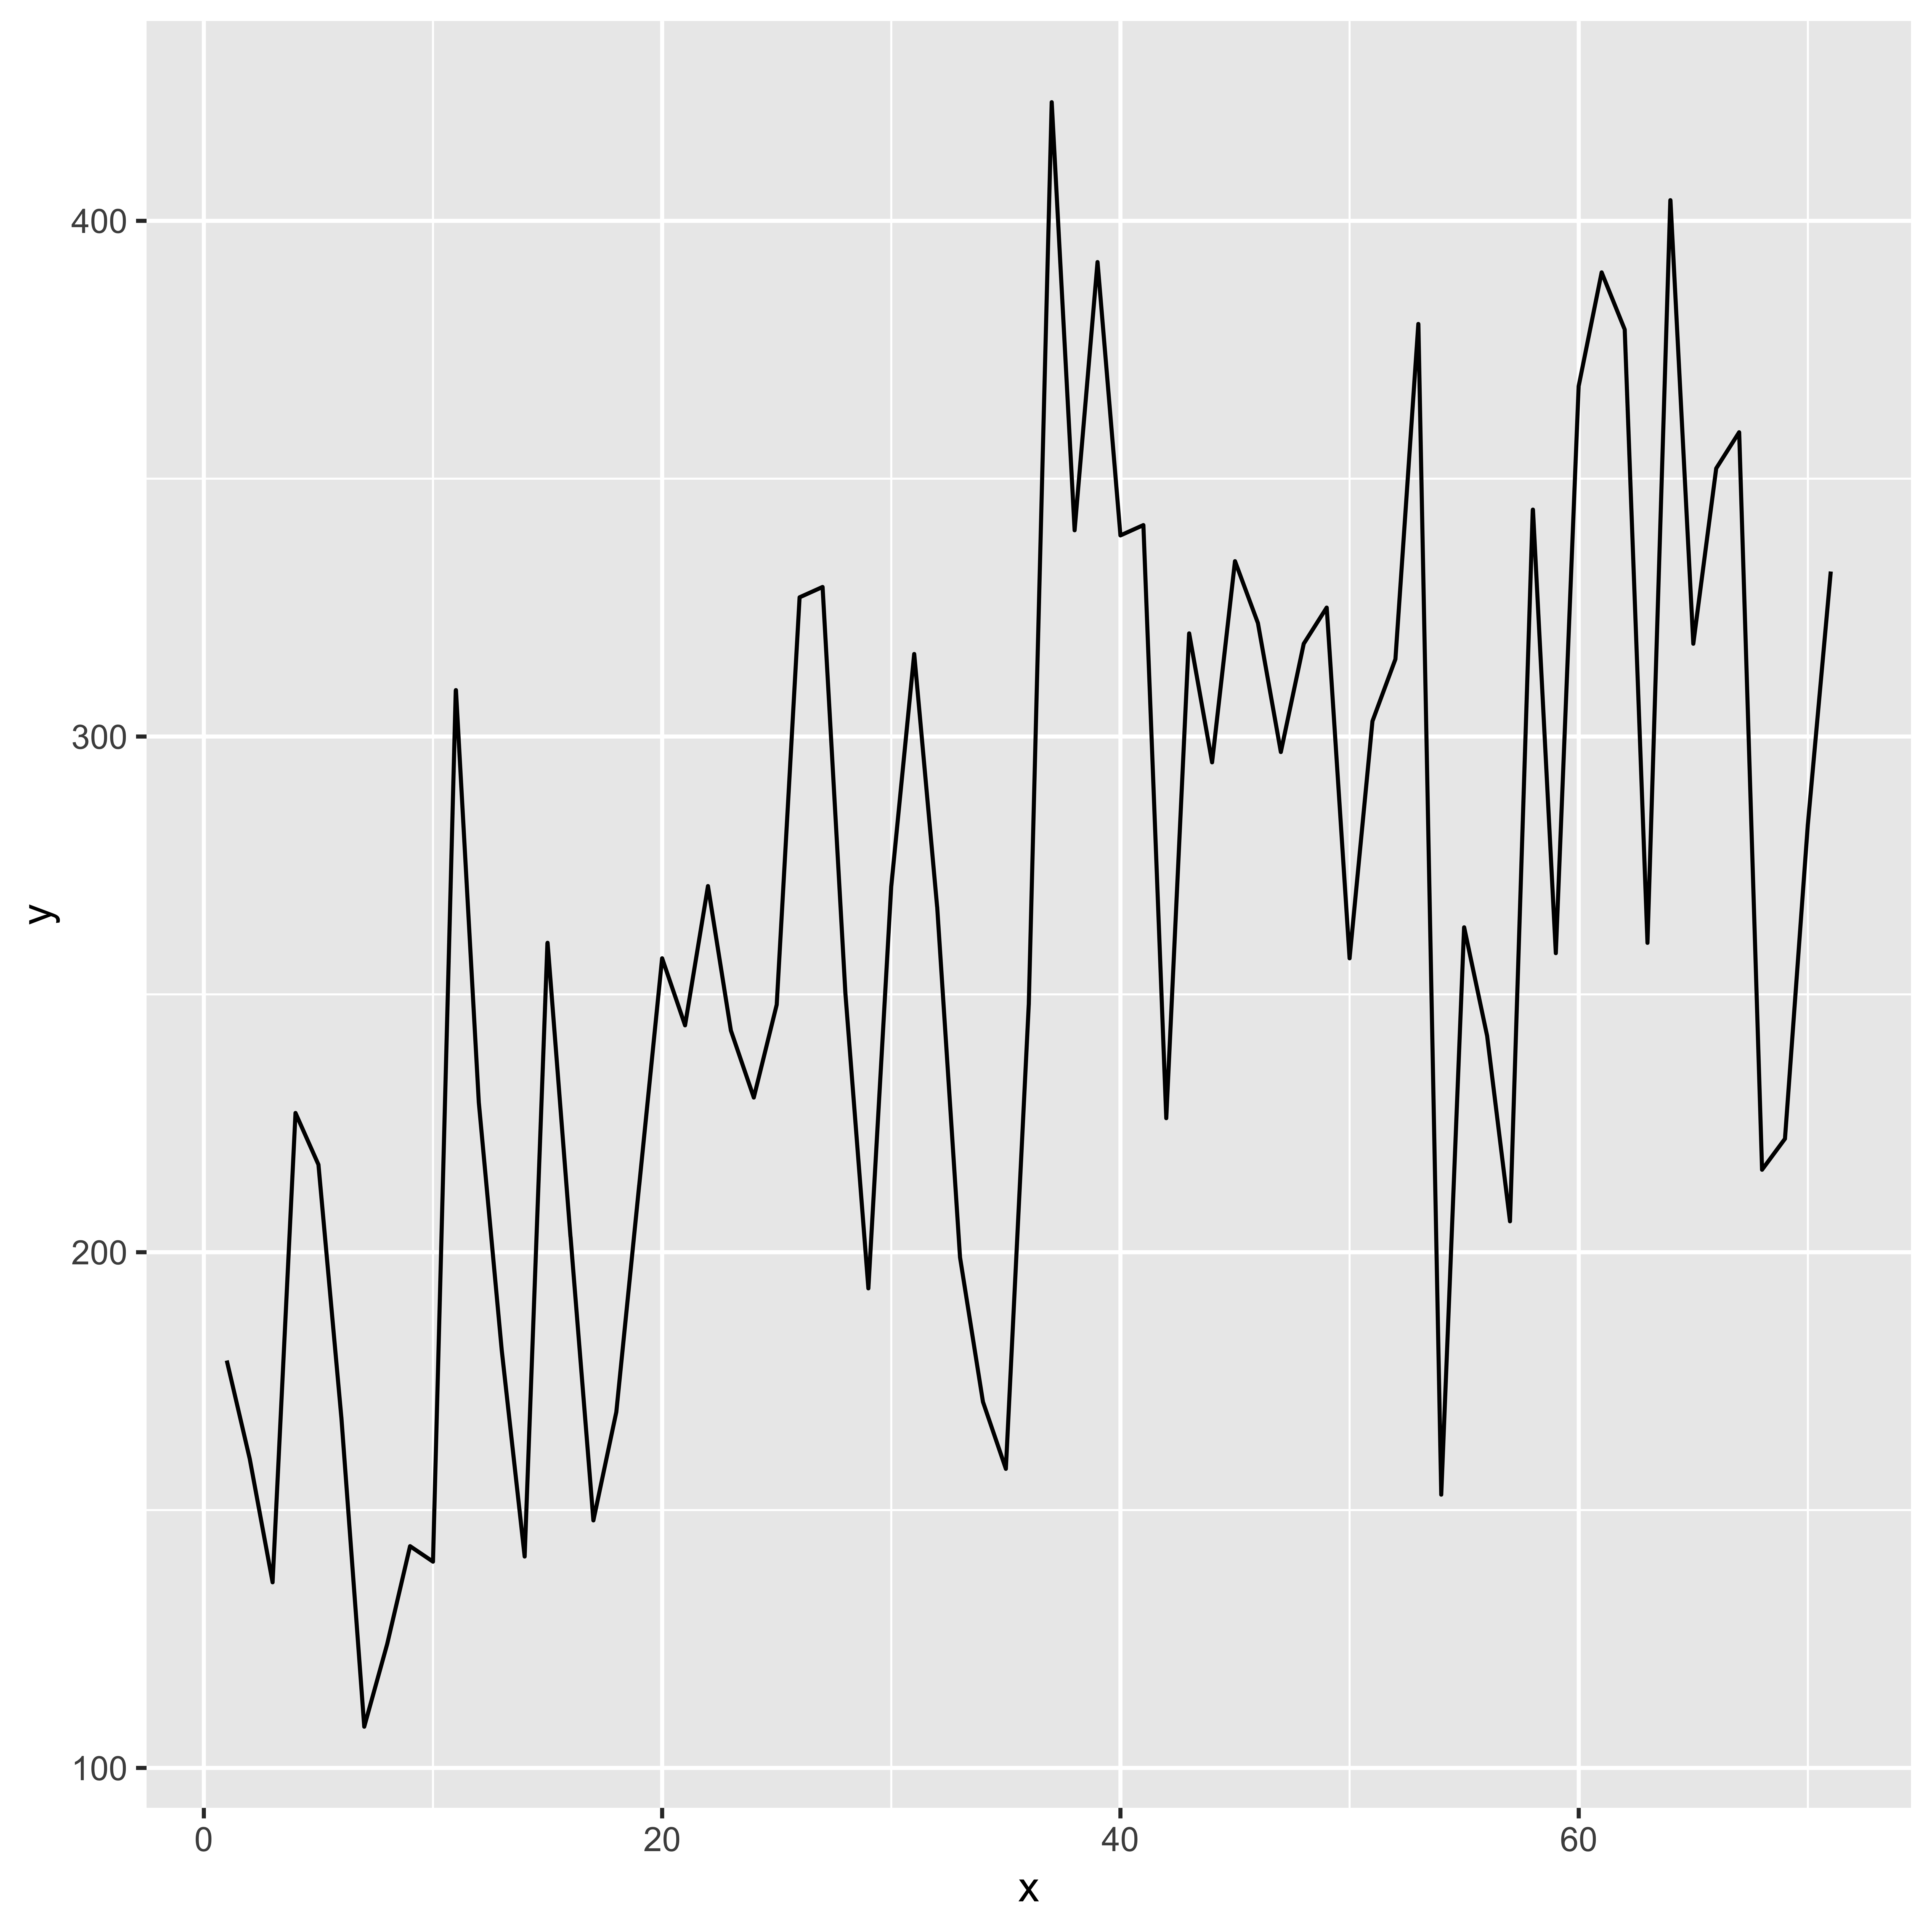
\includegraphics[width=\maxwidth]{figure/unnamed-chunk-7-1} 

}



\end{knitrout}


% latex table generated in R 3.5.3 by xtable 1.8-4 package
% Wed Sep 25 11:51:39 2019
\begin{table}[ht]
\centering
\begin{tabular}{rrrrr}
  \hline
 & Estimate & Std. Error & t value & Pr($>$$|$t$|$) \\ 
  \hline
(Intercept) & 179.13 & 15.04 & 11.91 & 0.00 \\ 
  x & 2.28 & 0.36 & 6.29 & 0.00 \\ 
   \hline
\end{tabular}
\caption{Оценки, которые мы заслужили!} 
\label{tab:regress}
\end{table}


Альтернативный способ оформлять таблицы

\begin{knitrout}
\definecolor{shadecolor}{rgb}{0.969, 0.969, 0.969}\color{fgcolor}\begin{kframe}
\begin{alltt}
\hlkwd{library}\hlstd{(dplyr)}
\hlstd{beautiful} \hlkwb{<-} \hlkwd{head}\hlstd{(chickwts)} \hlopt \hlkwd{kable}\hlstd{()}
\hlstd{x} \hlkwb{=} \hlnum{111111111111111111111111111111111111111111111111111111111111111111111111111111111111111111111111111111111111111111111111111111111111111111111111111111111111111111111111111111111111111111111111111111} \hlopt{+} \hlnum{22222}
\hlcom{# слишком длинные строки - оформление! }
\end{alltt}
\end{kframe}
\end{knitrout}

\begin{table}[h!]
\begin{center}

\begin{tabular}{r|l}
\hline
weight & feed\\
\hline
179 & horsebean\\
\hline
160 & horsebean\\
\hline
136 & horsebean\\
\hline
227 & horsebean\\
\hline
217 & horsebean\\
\hline
168 & horsebean\\
\hline
\end{tabular}


\caption{Стоимость акций}
\end{center} 
\end{table}


\begin{knitrout}
\definecolor{shadecolor}{rgb}{0.388, 0.749, 0.831}\color{fgcolor}\begin{kframe}
\begin{verbatim}
x <- rnorm(100)
x_mean <- mean(x)
if(x_mean > 40){
  text = 'Всё хорошо'
} else {
  text = 'Не очень'
}

x_mean = 6
\end{verbatim}
\end{kframe}
\end{knitrout}

Результат:  % Не очень

\section{Логические функцию}
6
\ifnumcomp{6}{>}{5}{ооушцуфо}{рашщрфцу}

\newbool{my_per}
\setbool{my_per}{true}

\ifbool{my_per}{публикую ответ}{не публикует ответ}

\end{document}


